
        \begin{abstract}{Modelling Supramolecular Polymers}{%
            B. Sundaram}{%
            JNCASR, Bengaluru}{%
            \KLtag}
        Unlike conventional polymers, supramolecular polymers are formed out of non-covalent interactions between monomers in solution. The relatively weaker interaction strengths makes the association between the monomers to be reversible. Molecular simulations are apt to study this self-assembly process as they possess the right tools to take into account finite temperature and bulk solvent conditions explicitly. The talk will review the vast experimental literature on this topic and will introduce the computational techniques. The application of such methods have led to the following new findings: ground state dipole configuration in the classic BTA system, dipole driven cooperative mechanism of polymerisation, reversal of chiral handedness concomitant with polarization reversal in ferroelectric thin films of supramolecular polymers, and the demonstration of isodesmicity in self-assembly, using free energy methods. \begin{center}  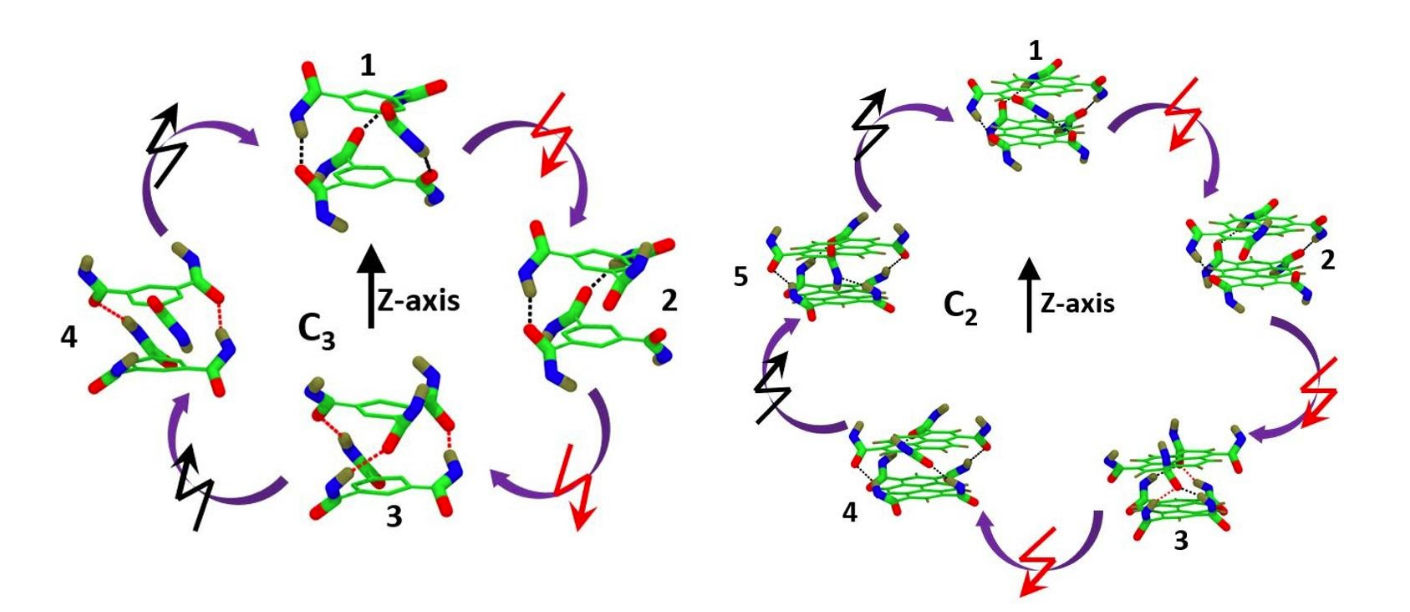
\includegraphics[width=\linewidth]{abstracts/txt/figures/bala.png}  \end{center}  
        \end{abstract}
        